\documentclass[]{article}

\usepackage{graphicx} \usepackage{amsmath} \usepackage{amssymb} \usepackage{caption}
\usepackage{hyperref} \usepackage{float}

\title{When Zombie’s Attack!: Mathematical Modelling of an Outbreak of Zombie Infection}
\author{Glenn Galvizo}

\begin{document}

\maketitle

\section{Background}
World War Z, Resident Evil, I Am Legend... these are all movies depicting the
outcome of a zombie outbreak. In almost all zombies movies, humanity is severely
diminished. The central plot is typically to search for this “cure” which turn our zombies
back to humans- but is finding the cure the right approach? Does quarantine work in
practice? Will the zombie population ever be completely eradicated? These are questions
that this paper tries to address, as they simulate the outbreak with modified SIR
models.

There are five scenarios that this paper goes over:
\begin{enumerate}
    \item  Susceptible population immediately becomes a zombie
    \item Susceptible population has a latent period before becoming a zombie
    \item Zombies and infected population are partially quarantined
    \item Zombies can be cured and become susceptible again
    \item Frequent and increasingly stronger attacks against zombies
\end{enumerate}

\section{Basic Zombie Model}
There exist three classes here: the susceptibles $S$, the zombies $Z$, and the
removed $R$ (i.e. dead). The figure for which these classes interact is given 
below:

\begin{figure}[H]
    \centering{
        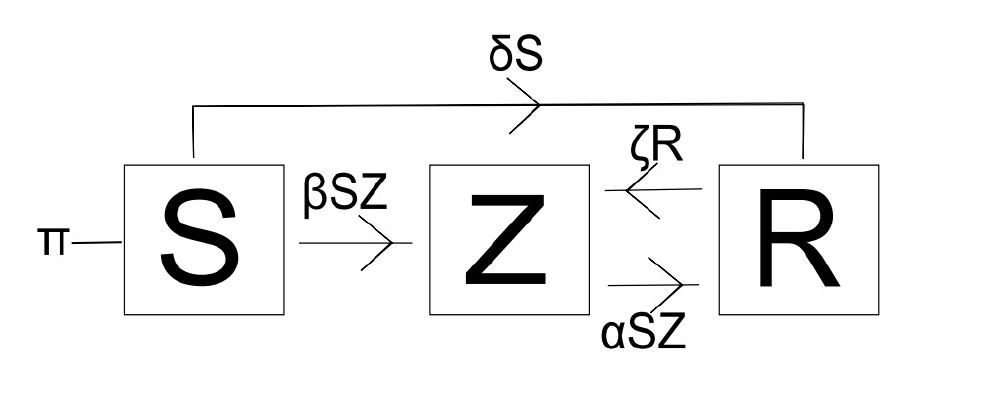
\includegraphics[scale=0.4]{images/basicmodel-diagram}
        \caption{
            Depicts the basic zombie model.
        }
    }
\end{figure}

If there are no zombies and no removed, then our $S$ population remains constant. This is depicted on the left in~\autoref{fig:basicmodel}.
With just one zombie, our $S$ population quickly declines to extinction in 5 timesteps. This is as the paper describes, with the parameters $\alpha = 0.005, \zeta = 0.0095, \zeta = 0.0001$, and $\delta = 0.0001$.

\begin{figure}[H]
    \centering{
        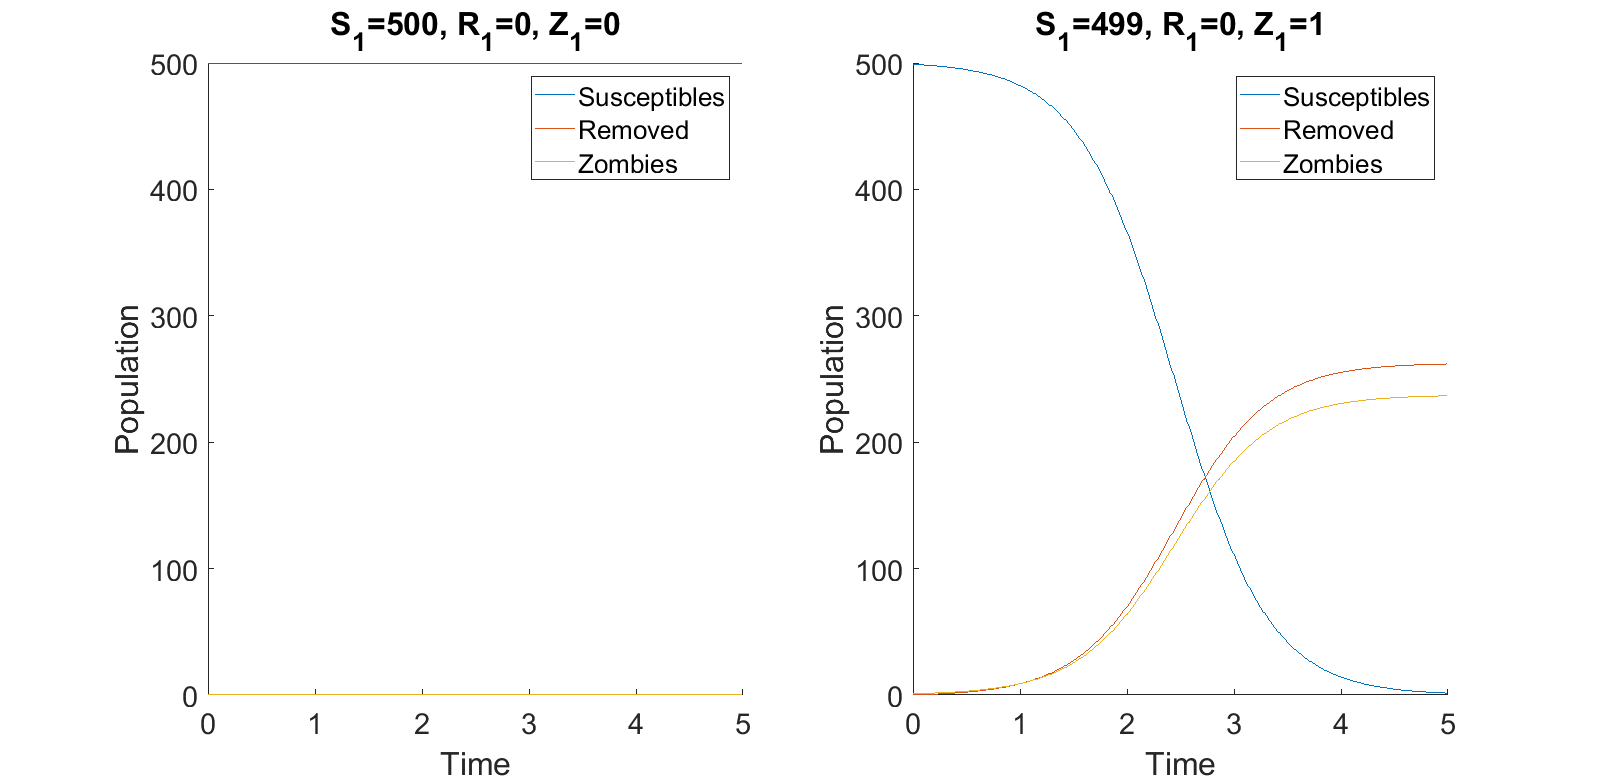
\includegraphics[scale=0.25]{images/basicmodel}
        \caption{
           Depicts case without zombie outbreak on left. Depicts case with zombie outbreak $(Z(1) = 1)$ on right. 
        }\label{fig:basicmodel}
    }
\end{figure}

What is not shown is the right graph in~\autoref{fig:basicmodel} is the slow approach to our all zombies steady state. In this mode, all individuals will eventually become zombies.

\section{Latent Infection Zombie Model}
We extend the basic model by including an infected class for those who "lose" an encounter with a zombie, but are not yet a zombie themselves. There exist four classes here: the susceptibles $S$, the infected $I$, the zombies $Z$, and the removed $R$. The figure for which these classes interact is given below:

\begin{figure}[H]
    \centering{
        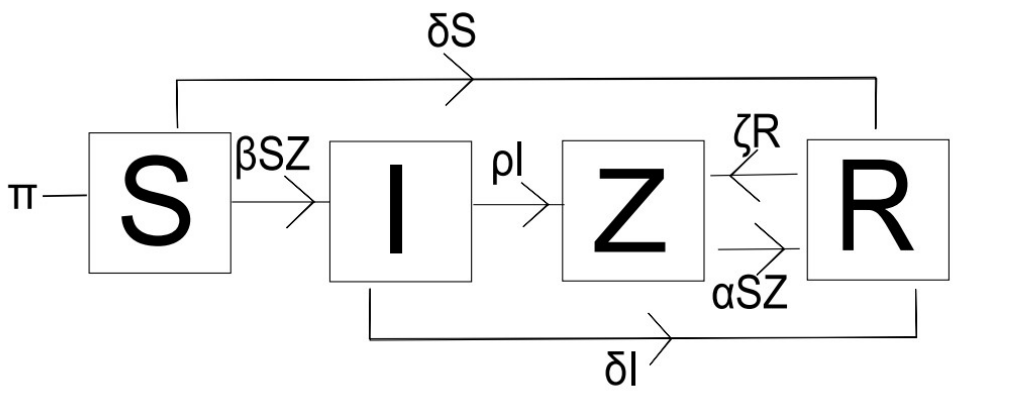
\includegraphics[scale=0.4]{images/latentinfectionmodel-diagram}
        \caption{
            Depicts the latent infection model.    
        }
    }
\end{figure}

Using the same parameters as before with $\rho = 0.00$, we note that an outbreak of one zombie causes a significant delay in our system toward the extinction of our susceptibles. The paper mentions that this period (which I denote as $t_e$) should be close to double the time in the basic model $t_e \simeq 6$, but my results show that this number is closer to $t_e \simeq 1000$. I could not replicate the original author's results without using unrealistic parameters (i.e.\ $> 1$).

\begin{figure}[H]
    \centering{
        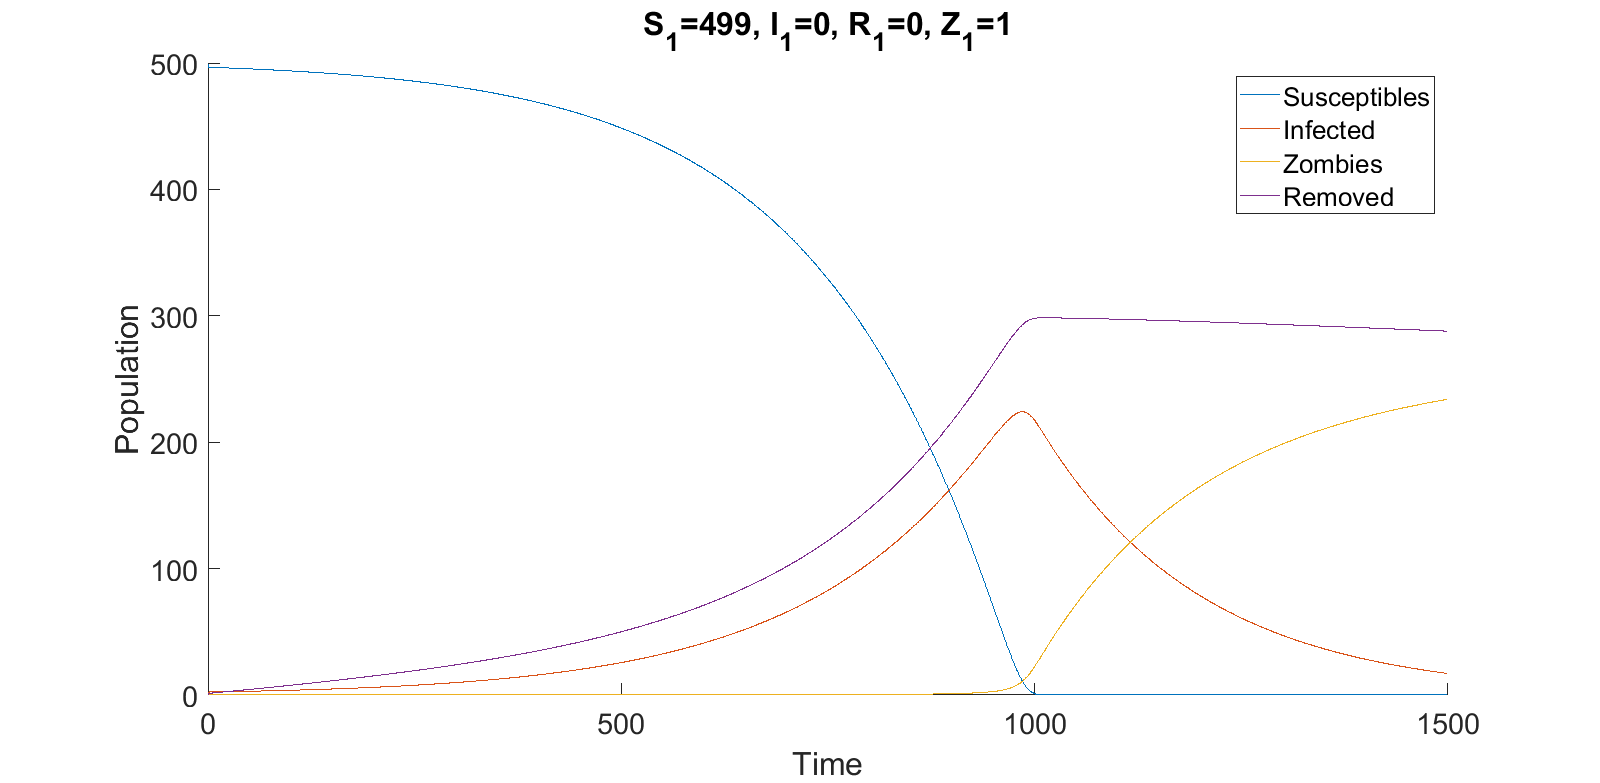
\includegraphics[scale=0.25]{images/latentinfectionmodel}
        \caption{
            Depicts the case of zombie outbreak using the latent infection model.
        }
    }
\end{figure}

From $0 < t < t_e$ our removed and infected progressively gets larger, while the
susceptibles get progressively smaller. The zombie population is very small during this
period, with values under the initial value of $Z = 1$. What I find interesting here is the
drastic changes for all classes around the $t = t_e$ mark. With all our susceptibles gone,
there’s no one to be infected anymore. With less individuals being infected, our removed
class steadily declines and our system approaches the steady state of all zombies again.

\section{Quarantine Zombie Model}
We extend our latent infection model by including a quarantine class to store a
fraction of the infected and zombie population. There exist five classes here: the
susceptibles $S$, the infected $I$, the zombies $Z$, the quarantined $Q$, and the removed $R$.
The figure for which these class interact is given below.

\begin{figure}[H]
    \centering{
        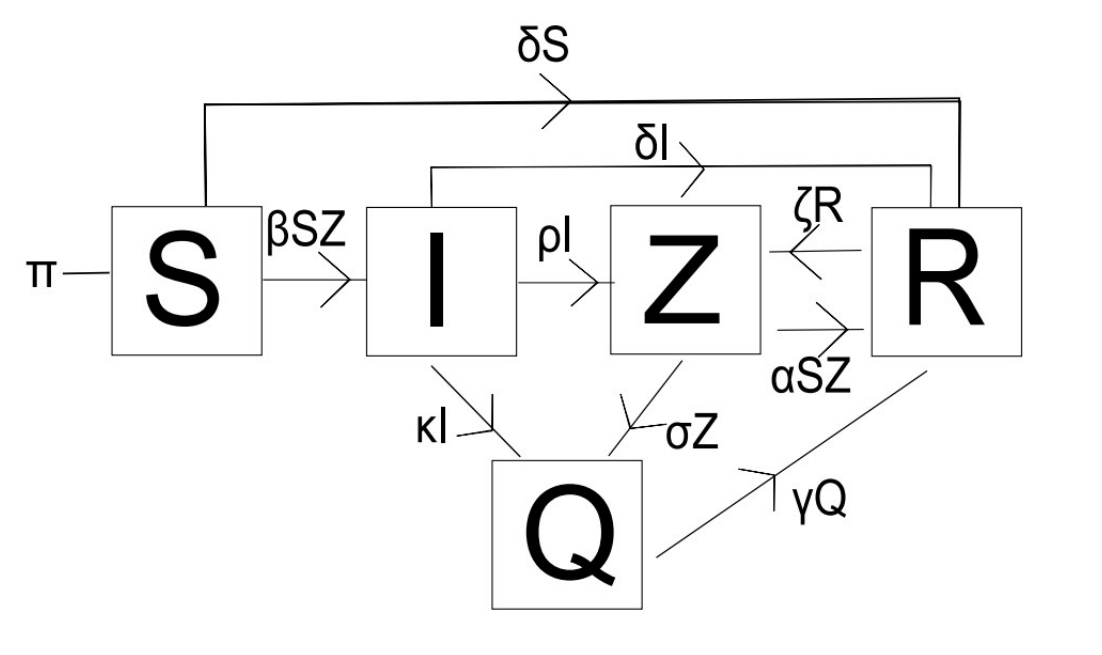
\includegraphics[scale=0.4]{images/quarentinemodel-diagram}
        \caption{
            Depicts the quarantine model.
        }
    }
\end{figure}

There are three new parameters introduced, two of which ($\kappa$ and $\sigma$)
must satisfy the following equation to lead to susceptible extinction:
\begin{equation}
    R_0 = \frac{\beta N \rho} {(\rho + \kappa)(\alpha N + \sigma)} > 1
\end{equation}
I used $\gamma = 0.003$, $\kappa = 0.003$, and $\sigma = 0.00003$, which gave me $R_0 = 1.86077 > 1$ if we keep the other parameters the same as before. We note that our time to susceptible extinction is extended again, which the paper does state- but they have extinction times $t_e \simeq 20$, as opposed to here with a time closer to $t_e \simeq 1750$.

\begin{figure}[H]
    \centering{
        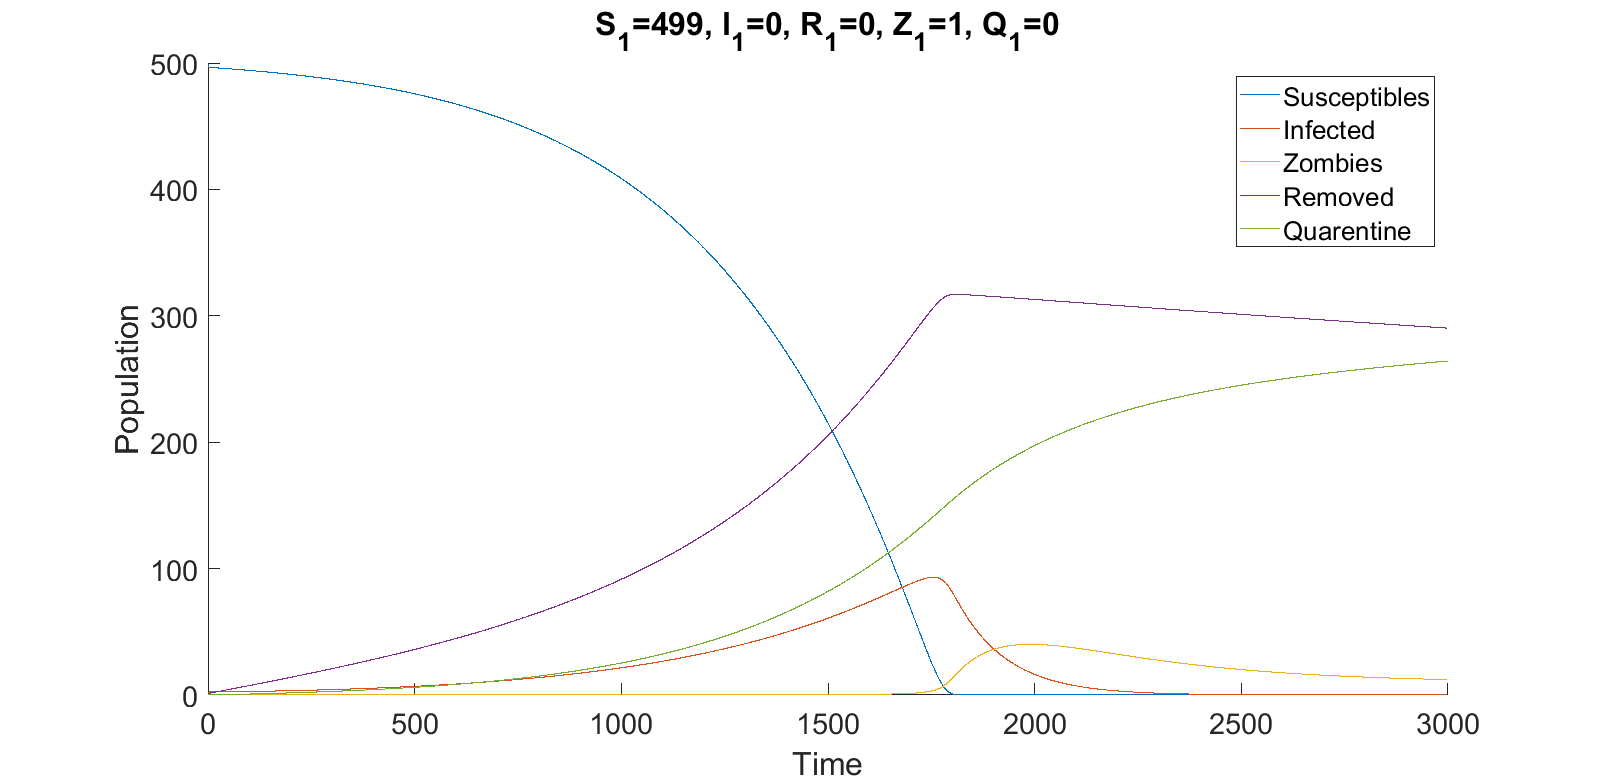
\includegraphics[scale=0.25]{images/quarentinemodel}
        \caption{
            Depicts case of zombie outbreak using quarentine model with $R_0 > 1$.
        }
    }
\end{figure}

Like our latent infection model, we observe similar effects from $0 < t < t_e$ . The
susceptibles rapidly decline, our zombies reside near extinction, and our infected and
removed rapidly increase. We note that our quarantine rapidly increases during this
period as well. For $t > t_e$ , our quarantine, removed, and zombie populations approach
their respective stable values. It is interesting to note here that we no longer have a
steady state of all zombies, but rather it is composed of zombies, removed, and
quarantined.
The paper states that if our basic reproductive ratio $R_0$ is less than one, than our
disease-free equilibrium is stable. I used the same parameters as the latent infection
model does, with $\gamma = 0.00003$, $\kappa = 0.3$, and $\sigma = 0.000003$ to get $R_0 = 0.031148 < 1$.
My observations go against what the paper states, which is that we retain our
susceptible population.

\begin{figure}[H]
    \centering{
        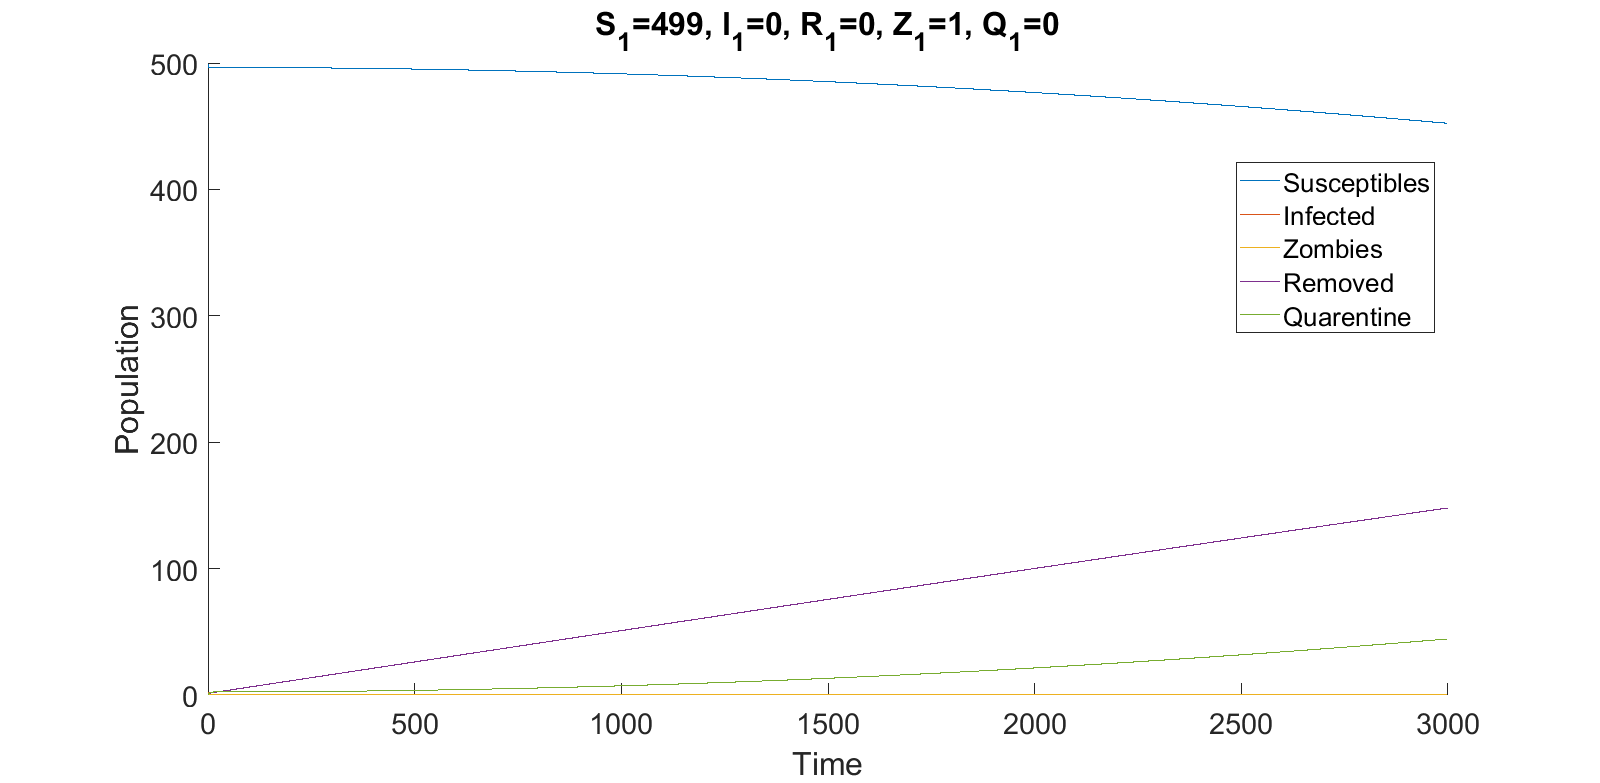
\includegraphics[scale=0.25]{images/quarentinemodel-no-zombies}
        \caption{
            Depicts case of zombie outbreak using quarentine model with $R_0 < 1$.
        }
    }
\end{figure}

In the figure above, we observe that our zombies and infected individuals exist in very
small quantities, our susceptibles decline slowly, and our removed and quarantine
population increase slowly. What this figure really shows is a section of an elongated a
graph like figure 6. The susceptibles eventually reach extinction, and our zombie,
removed, and quarantine populations remain.

\section{Treatment Zombie Model}
We extend our latent infection model by allowing a portion of our zombie class to
move back to our susceptible class. There exist four classes here: the susceptibles $S$, the
infected $I$, the zombies $Z$, and the removed $R$. The figure for which these class interact
is given below.
\begin{figure}[H]
    \centering{
        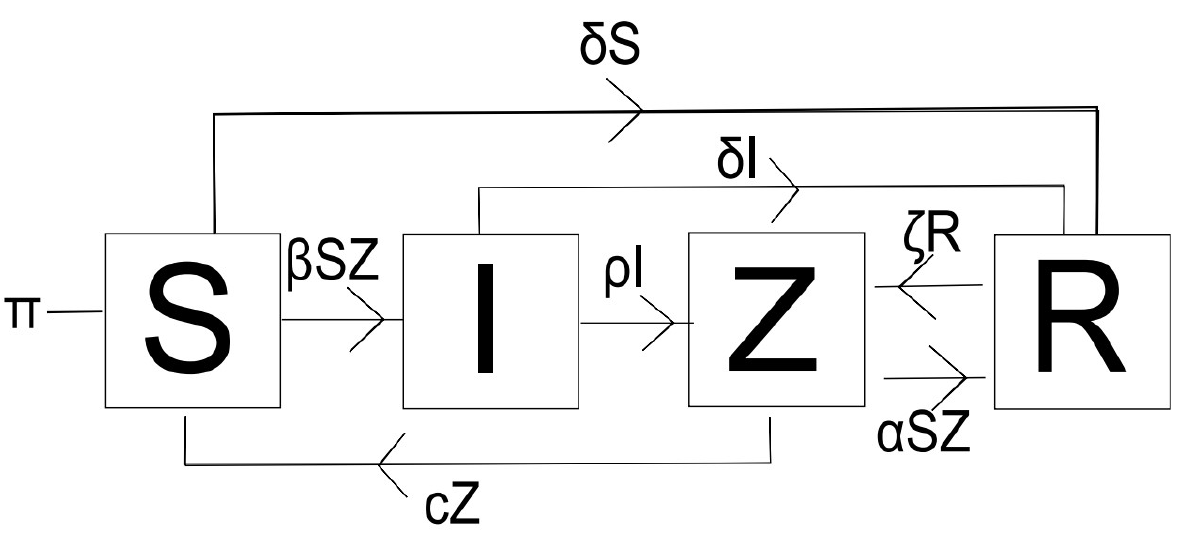
\includegraphics[scale=0.4]{images/curemodel-diagram}
        \caption{
            Depicts the treatment model.
        }
    }
\end{figure}

We use the same parameters as the latent infection model, and choose $c = 0.05$
arbitrarily. The paper states that coexistence between zombies and susceptibles are
possible here, but susceptibles will exist in sparse numbers. I compute the exact same
results as the paper suggests, with a final susceptible population $\bar{S̅}= 5.2632$.
\begin{figure}[H]
    \centering{
        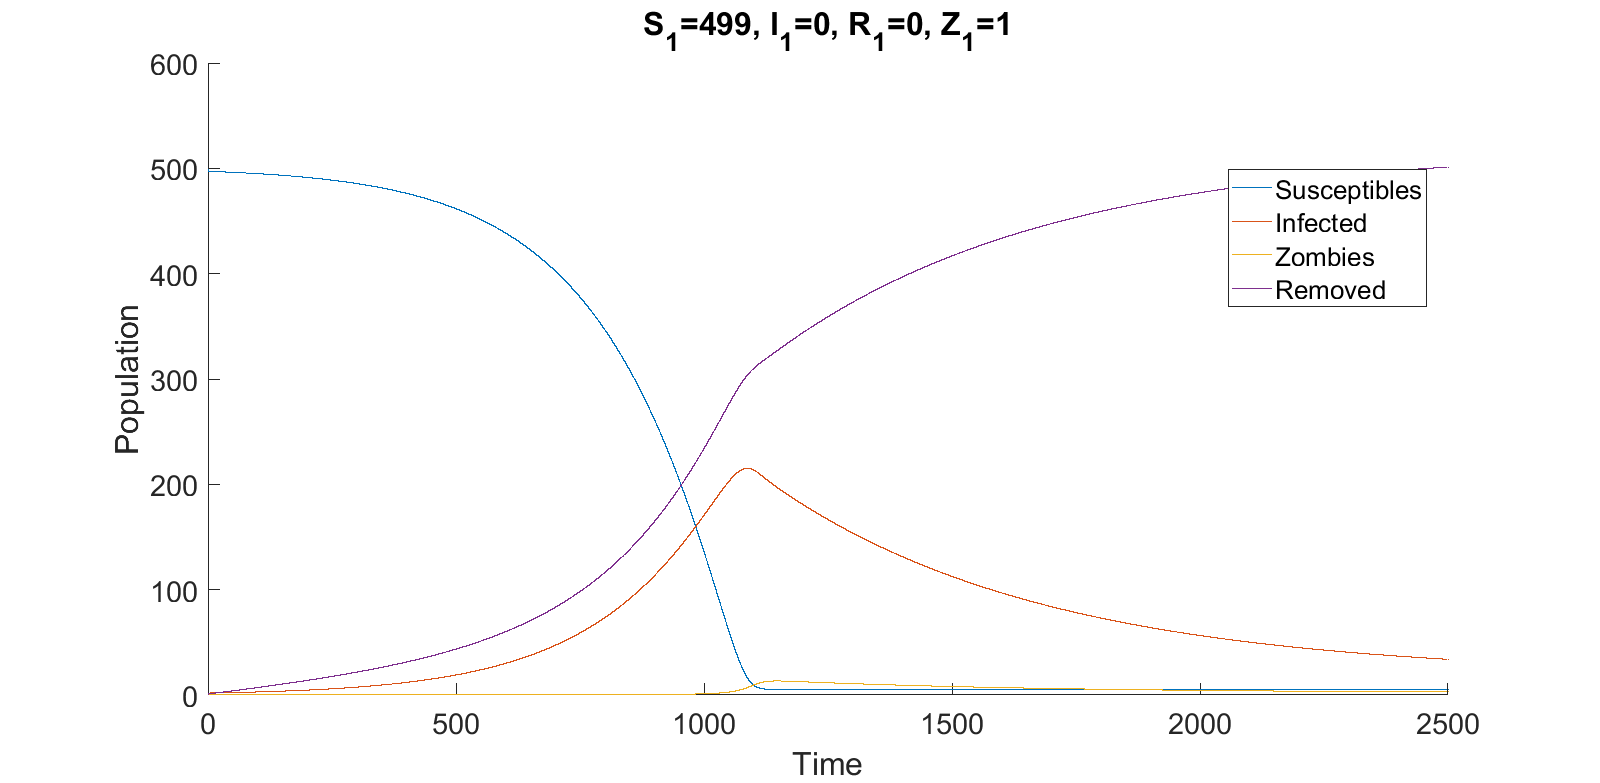
\includegraphics[scale=0.25]{images/curemodel}
        \caption{
            Depicts case of zombie outbreak using treatment model.
        }
    }
\end{figure}
The authors state that our steady state $(\bar{S}, \bar{I}, \bar{Z}, \bar{R})$ is as follows:
\begin{equation}
    \begin{aligned}
        \bar{S} &= \frac{c}{\beta} = 5.2632 \\
        \bar{I} &= \frac{c}{\rho} \bar{Z} = 10 \cdot \bar{Z} \\
        \bar{Z} &= \bar{Z} \\
        \bar{R} &= \frac{\alpha \cdot c}{\zeta \cdot \beta} \bar{Z} = 263.1579 \cdot \bar{Z}
    \end{aligned}
\end{equation}
I do not observe these numbers in the same time interval as the paper, but I do observe these exact numbers with $\bar{Z} = 1.9106$.

\section{Impulsive Eradication Zombie Model}
We extend our basic model by including waves of eradication of the zombie class.
Here, we just attempt to kill more and more zombies with every eradication attempt. I
did not use the parameters they specified in the paper, as I obtained a differently shaped
curve (parabolic and a sparse population). To mimic their results best, I used $\alpha =
0.0055, \beta = 0.0095, \zeta = 0.0001 \delta = 0.0001, \kappa = 0.25$, and a time period $T = 20$, I
obtain the results below.

\begin{figure}[H]
    \centering{
        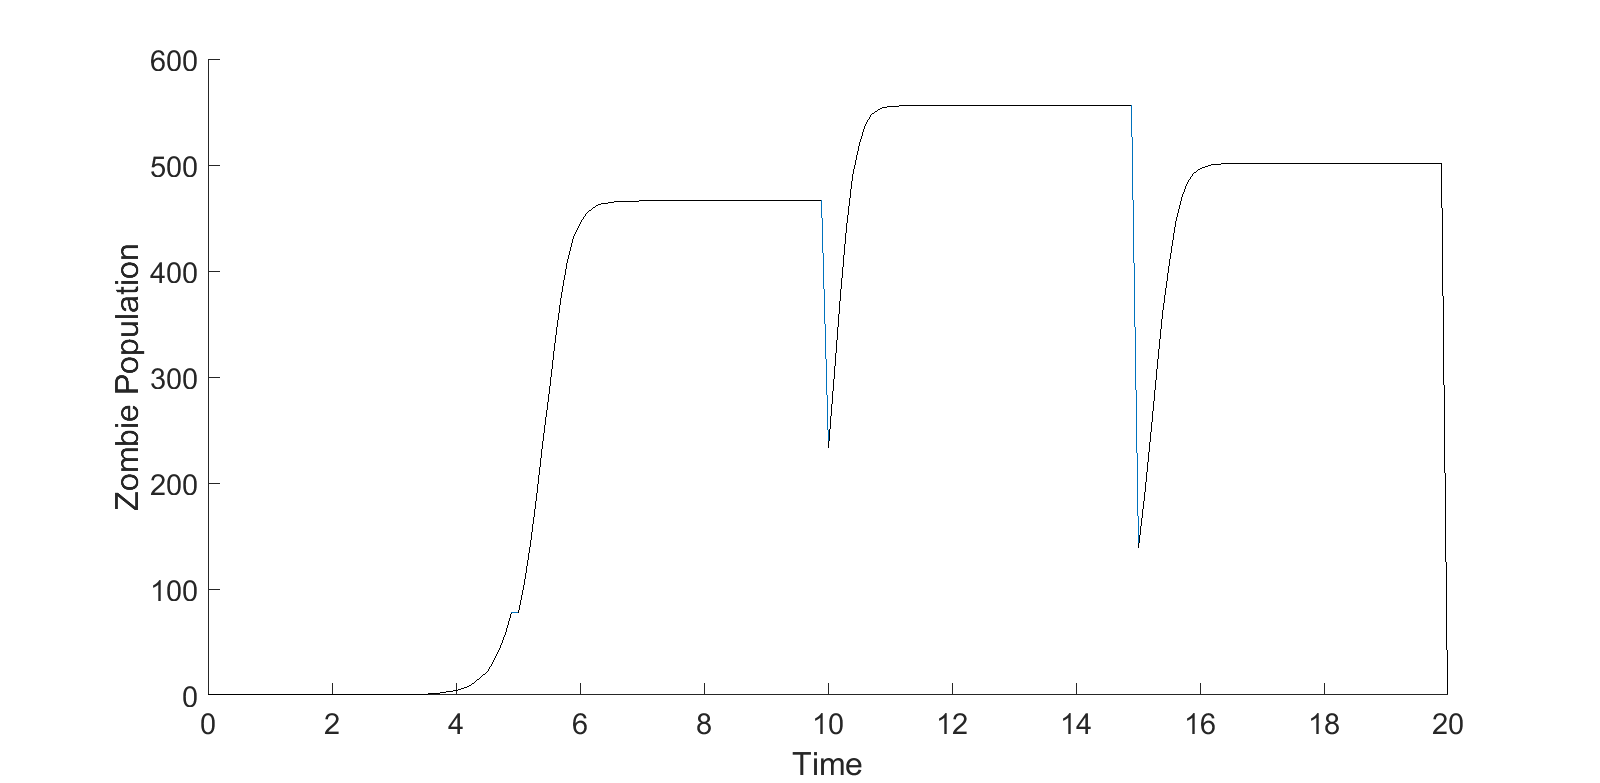
\includegraphics[scale=0.25]{images/eradication}
        \caption{
            Depicts zombie outbreak using impulsive zombie eradication.
        }
    }
\end{figure}
With a starting population of $S(1) = 1000$, our zombie population never grows past 600.
The paper has the same starting $S(1) = 1000$ population, but their zombies grow to a
1000. The first kill wave is at $t = 5$, and the outcome isn’t very successful at this point
with no decline in $Z$. Our second kill wave at $t = 10$ eradicates roughly 200 zombies.
Our third kill wave at $t = 15$ eradicates twice as much zombies as our second kill wave.
And finally, all our zombies are eradicated at the end of time period.

The conclusion they arrive to in the paper is that the only way to truly eradicate the
zombie population is with this impulsive eradication.

\section{Permanent Zombie Disable Model}
resurrection. In popular zombie media, a common method for permanently disabling a
zombie is to take its head off. The paper states that this action moves them to removed
class, which allows them to turn into a zombie again- but we will extend this model by
creating a separate class for this. We will also consider where a susceptible eradicates
the inevitable zombification of an infected individual.
The latent infection model is extended by adding a class  for eradicated and
is with this impulsive eradication.

The latent infection model is extended by adding a class $E$ for eradicated and
parameters $\epsilon_1, \epsilon_2$ to indicate that a zombie or infected person has been eradicated. This
gives us the following ODEs:
\begin{equation}
    \begin{aligned}
        S' &= \Pi - \beta S Z - \delta S \\
        I' &= \beta S Z - \rho I - \delta I - \epsilon_1 S I \\
        Z' &= \rho I + \zeta R - \alpha S Z - \epsilon_2 S Z \\
        R' &= \delta S + \delta I + \alpha S Z - \zeta R \\
        E' &= \epsilon_1 S I + \epsilon_2 S Z
    \end{aligned}
\end{equation}
To analyze this model, I used Euler’s method for approximatel ODEs. This is the
same method used in the paper to analyze our previous models. Using the same
parameters as our latent infection model and $\epsilon_1 = 0.0002, \epsilon_2 = 0.004$ (there are more
zombies being eradicated than infected), we get the figure below.
\begin{figure}[H]
    \centering{
        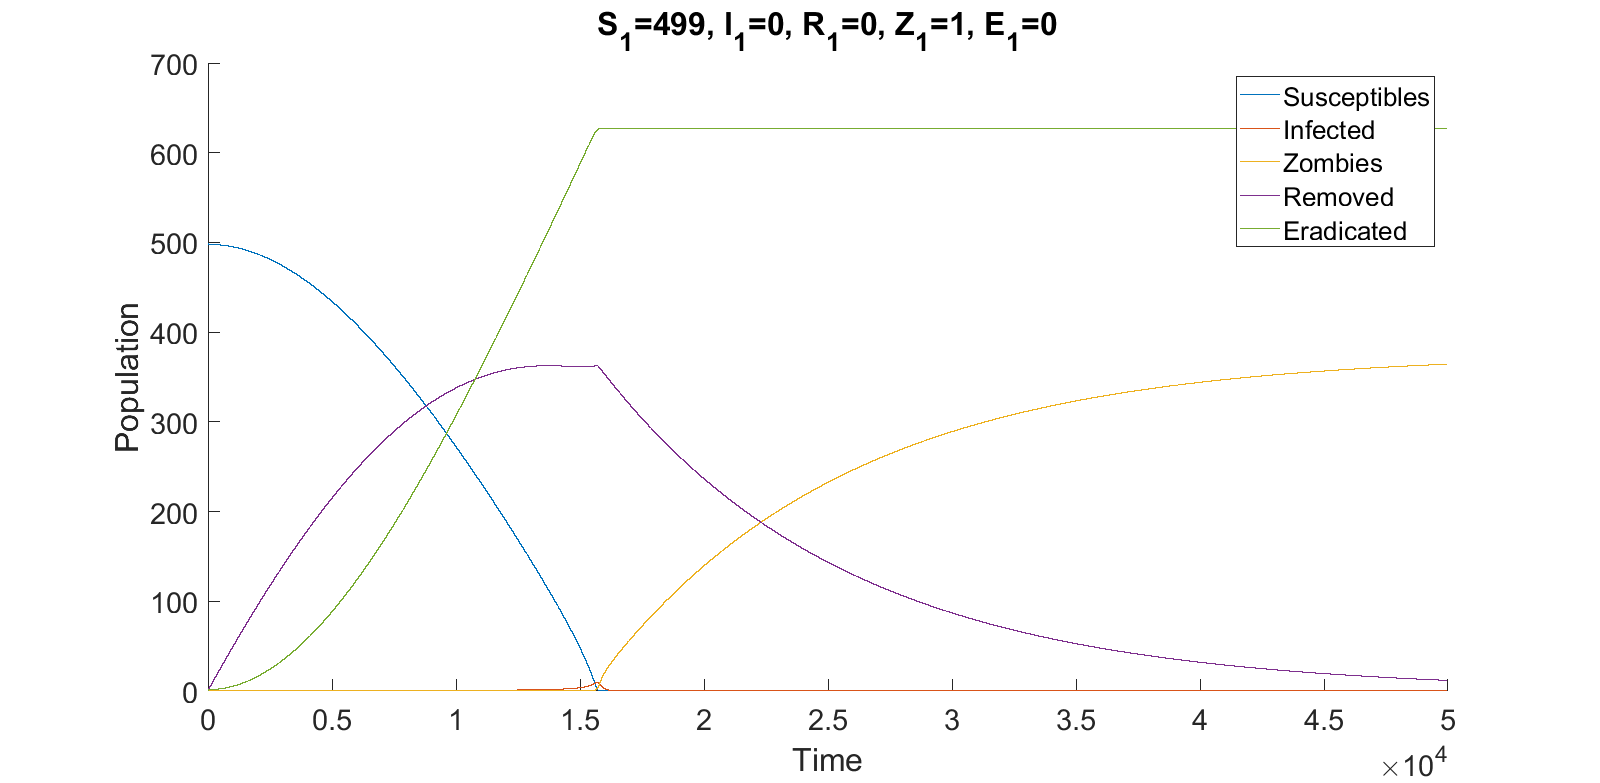
\includegraphics[scale=0.25]{images/deathmodel}
        \caption{
            Depicts zombie outbreak using permanent zombie disable model.
        }
    }
\end{figure}
Our system eventually moves the steady state of only zombies, but over a long time. It
takes $t = 1.5 \cdot 10^4$ periods for our starting susceptible population of 500 to reach
extinction.

From $0 < t < t_e$ , our susceptible population declines, our zombie and infected remain
close to extinction, and the removed and eradicated population increases. The infected
population is only seen for a brief moment, as our susceptibles become extinct. As soon
as our susceptible population reaches extinct, there is no one to kill the zombies. This
leads to a constant population in $E$ for $t > t_e$ .

\section{Conclusion}
We went over six models for modeling zombie outbreaks, of which two (the
treatment and impulsive eradication models) allow our susceptible population to live. I
was not able to replicate the exact results of the models past the basic model, but most
of their conclusions (except for the quarantine model) held true. Indeed, the best
method for dealing with a zombie outbreak is to impulsively eradicate the zombies.

\end{document}



